\section{\large Ejercicio 3. Aplicación de los sistemas de ecuaciones lineales en la resolución de problemas básicos.}

Enuncie el sistema de ecuaciones lineales que describe la problemática y resuelva utilizando el método de reducción de Gauss-Jordán. Se recomienda emplear GeoGebra u otra herramienta como la calculadora de matrices para resolver el sistema de ecuaciones lineales. 

\textbf{Enunciado:} Una persona invirtió un total de \$20,000 en tres inversiones al 6, 8 y 10\%. El ingreso anual total fue de \$1624 y el ingreso de la inversión del 10\% fue dos veces el ingreso de la inversión al 6\%. ¿De cuánto fue cada inversión?

\begin{center}
    \textbf{Sistema de ecuaciones identificada}
\end{center}

\[
    \begin{cases}
        \begin{array}{l}
            0.06x+0.08y+0.10z=1624 \\
            0.12x-0.10z=0 \\
            x+y+z=20000 \\    
        \end{array}
    \end{cases}
\]

\begin{figure}[ht!]
    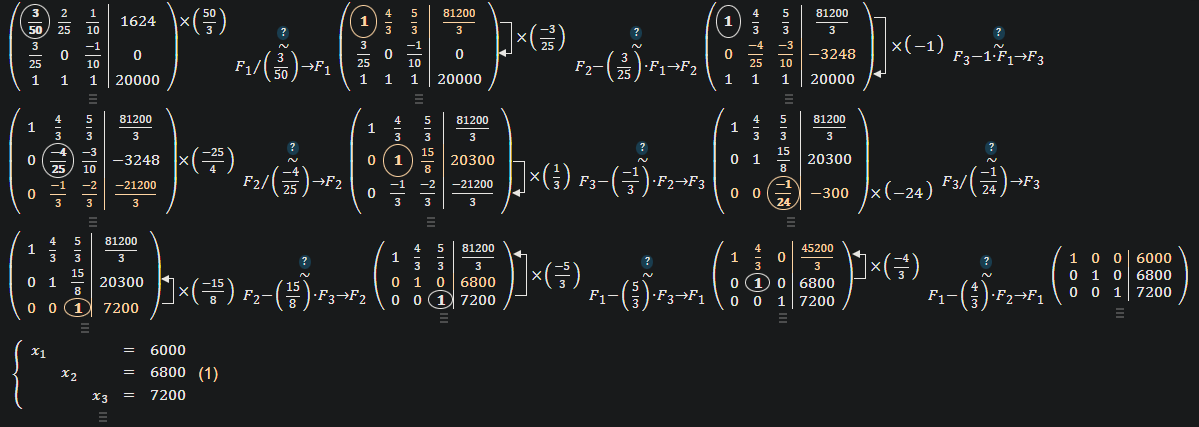
\includegraphics[width=\textwidth, height=300pt]{calculadora-de-matrizes1.png}
\end{figure}

\begin{center}
    \textbf{Solución:} \(\left(600,6800,7200\right)\)
\end{center}